\begin{pages}
    \begin{Rightside}
    \selectlanguage{greek}
        \beginnumbering
        \pstart[
        			\chapter{Ὁ τῆς ζωῆς ποταμός}
        			\markboth{The River of Life}
				]
		\renewcommand{\LettrineFontHook}{\PHtitl}
		\lettrine[lines=3]{Κ}{αὶ} ἔδειξέν μοι ποταμὸν ὕδατος ζωῆς λαμπρὸν ὡς κρύσταλλον, ἐκπορευόμενον ἐκ τοῦ θρόνου τοῦ Θεοῦ καὶ τοῦ Ἀρνίου. ἐν μέσῳ τῆς πλατείας αὐτῆς καὶ τοῦ ποταμοῦ ἐντεῦθεν καὶ ἐκεῖθεν ξύλον ζωῆς ποιοῦν καρποὺς δώδεκα, κατὰ μῆνα ἕκαστον ἀποδιδοῦν τὸν καρπὸν αὐτοῦ, καὶ τὰ φύλλα τοῦ ξύλου εἰς θεραπείαν τῶν ἐθνῶν. 
		\pend
		\pstart
		καὶ πᾶν κατάθεμα οὐκ ἔσται ἔτι. καὶ ὁ θρόνος τοῦ Θεοῦ καὶ τοῦ Ἀρνίου ἐν αὐτῇ ἔσται, καὶ οἱ δοῦλοι αὐτοῦ λατρεύσουσιν αὐτῷ, καὶ ὄψονται τὸ πρόσωπον αὐτοῦ, καὶ τὸ ὄνομα αὐτοῦ ἐπὶ τῶν μετώπων αὐτῶν. καὶ νὺξ οὐκ ἔσται ἔτι, καὶ οὐκ ἔχουσιν χρείαν φωτὸς λύχνου καὶ φωτὸς ἡλίου, ὅτι Κύριος ὁ Θεὸς φωτίσει ἐπ’ αὐτούς, καὶ βασιλεύσουσιν εἰς τοὺς αἰῶνας τῶν αἰώνων.
		\pend
		\pstart
		Καὶ εἶπέν μοι Οὗτοι οἱ λόγοι πιστοὶ καὶ ἀληθινοί, καὶ ὁ Κύριος ὁ Θεὸς τῶν πνευμάτων τῶν προφητῶν ἀπέστειλεν τὸν ἄγγελον αὐτοῦ δεῖξαι τοῖς δούλοις αὐτοῦ ἃ δεῖ γενέσθαι ἐν τάχει. καὶ Ἰδοὺ ἔρχομαι ταχύ. μακάριος ὁ τηρῶν τοὺς λόγους τῆς προφητείας τοῦ βιβλίου τούτου. Κἀγὼ Ἰωάννης ὁ ἀκούων καὶ βλέπων ταῦτα. καὶ ὅτε ἤκουσα καὶ ἔβλεψα, ἔπεσα προσκυνῆσαι ἔμπροσθεν τῶν ποδῶν τοῦ ἀγγέλου τοῦ δεικνύοντός μοι ταῦτα. καὶ λέγει μοι Ὅρα μή· σύνδουλός σού εἰμι καὶ τῶν ἀδελφῶν σου τῶν προφητῶν καὶ τῶν τηρούντων τοὺς λόγους τοῦ βιβλίου τούτου· τῷ Θεῷ προσκύνησον. 
		\pend
		\pstart
		Καὶ λέγει μοι Μὴ σφραγίσῃς τοὺς λόγους τῆς προφητείας τοῦ βιβλίου τούτου· ὁ καιρὸς γὰρ ἐγγύς ἐστιν. ὁ ἀδικῶν ἀδικησάτω ἔτι, καὶ ὁ ῥυπαρὸς ῥυπανθήτω ἔτι, καὶ ὁ δίκαιος δικαιοσύνην ποιησάτω ἔτι, καὶ ὁ ἅγιος ἁγιασθήτω ἔτι. Ἰδοὺ ἔρχομαι ταχύ, καὶ ὁ μισθός μου μετ’ ἐμοῦ, ἀποδοῦναι ἑκάστῳ ὡς τὸ ἔργον ἐστὶν αὐτοῦ. ἐγὼ τὸ Ἄλφα καὶ τὸ Ὦ, ὁ πρῶτος καὶ ὁ ἔσχατος, ἡ ἀρχὴ καὶ τὸ τέλος. μακάριοι οἱ πλύνοντες τὰς στολὰς αὐτῶν, ἵνα ἔσται ἡ ἐξουσία αὐτῶν ἐπὶ τὸ ξύλον τῆς ζωῆς καὶ τοῖς πυλῶσιν εἰσέλθωσιν εἰς τὴν πόλιν. ἔξω οἱ κύνες καὶ οἱ φάρμακοι καὶ οἱ πόρνοι καὶ οἱ φονεῖς καὶ οἱ εἰδωλολάτραι καὶ πᾶς φιλῶν καὶ ποιῶν ψεῦδος.
		\pend
		\pstart
		Ἐγὼ Ἰησοῦς ἔπεμψα τὸν ἄγγελόν μου μαρτυρῆσαι ὑμῖν ταῦτα ἐπὶ ταῖς ἐκκλησίαις. ἐγώ εἰμι ἡ ῥίζα καὶ τὸ γένος Δαυείδ, ὁ ἀστὴρ ὁ λαμπρός, ὁ πρωϊνός. Καὶ τὸ Πνεῦμα καὶ ἡ νύμφη λέγουσιν Ἔρχου. καὶ ὁ ἀκούων εἰπάτω Ἔρχου. καὶ ὁ διψῶν ἐρχέσθω, ὁ θέλων λαβέτω ὕδωρ ζωῆς δωρεάν.
		\pend
		\pstart
		Μαρτυρῶ ἐγὼ παντὶ τῷ ἀκούοντι τοὺς λόγους τῆς προφητείας τοῦ βιβλίου τούτου· ἐάν τις ἐπιθῇ ἐπ’ αὐτά, ἐπιθήσει ὁ Θεὸς ἐπ’ αὐτὸν τὰς πληγὰς τὰς γεγραμμένας ἐν τῷ βιβλίῳ τούτῳ· καὶ ἐάν τις ἀφέλῃ ἀπὸ τῶν λόγων τοῦ βιβλίου τῆς προφητείας ταύτης, ἀφελεῖ ὁ Θεὸς τὸ μέρος αὐτοῦ ἀπὸ τοῦ ξύλου τῆς ζωῆς καὶ ἐκ τῆς πόλεως τῆς ἁγίας, τῶν γεγραμμένων ἐν τῷ βιβλίῳ τούτῳ. Λέγει ὁ μαρτυρῶν ταῦτα Ναί, ἔρχομαι ταχύ. Ἀμήν, ἔρχου Κύριε Ἰησοῦ.
		\pend
		\pstart
		Ἡ χάρις τοῦ Κυρίου Ἰησοῦ μετὰ πάντων.	
		\pend
        \endnumbering
    \end{Rightside}
    \begin{Leftside}
        \beginnumbering
        \pstart[
        			\chapter{The River of Life}
				]		
		\renewcommand{\LettrineFontHook}{\Zallmanfamily}
		\lettrine[lines=3]{A}{nd} he showed me a river of water of life (and it was) as pure as a crystal; (and the river was) coming out of the throne of God and of the Lamb. And in the middle of its (the city’s) road, and from here and from there around the river (on either side / both sides of the river), there was a tree of life (which was) making (i. e. bearing) twelve (types of?) fruit; (and) each month it yields the according fruit (of that particular month) and its leaves are for the healing of the nations. 
		\pend
		\pstart
		And there will not be any (all) curses anymore. And the throne of God and the Lamb shall be therein (i. e. the city) and His servants will worship Him; and they will see His face and His name will be upon their foreheads. And night will be no longer and they will need neither the light of a lamp nor the light of the Sun, for the Lord God will shine (light) upon them — and they shall reign into the eternity of eternities (forever). 
		\pend
		\pstart
		And he (the angel) said to me, “These words are faithful and true and the Lord God sent His angel (which was one) of the holy prophets, to show His servants what must soon happen. ‘And behold! I will soon come!’ Blessed is the one who honours the words of the prophecy of this book.” And even I, John, was a listener and watcher of this (event). And when I heard and saw (these things), I fell (to my knees?) to worship before feet of the angel (who was) showing me this. And he tells me, “See not (i. e. do not do this)! I am your fellow servant and (I am also a fellow servant) of the prophets and of the ones honouring the words of this book — worship God (instead of me).”
		\pend
		\pstart
		And he says to me, “Do not seal the words of the prophecy of this book, for the time is near. He who does unjust things, let him do unjust things still; and let the defiler defile still; and let the just do justice still; and let the holy be holy still. ‘And behold, I am coming soon. And My reward (will come) with Me, to give to each how his work is (according to their deeds). I am the Alpha and the Omega, the first and the last, the beginning and the end.’ Blessed are those washing their robes, so that their authority may be upon the tree of life and by the gates they shall enter the city. Outside (of the city there are) the dogs and the sorcerers and the sexually immoral and the murderers and the ones worshipping idols and (also) everyone who likes or does false things.”
		\pend
		\pstart
		“I, Jesus, (have) sent my angel to testify to you that which concerns the churches. I am the root and the offspring of David — the bright morning star.” And the Spirit and the bride are saying, “Come. And he who hears, let him (also) say, ‘Come’. Let the thirsty come and let him who wishes (to) take from the water of life (do so freely).”
		\pend
		\pstart
		I testify to every listener of the words of the prophecy of this book; (and) if someone places upon them (adds something to them), God will put upon him the plagues which are written in this book. And if someone takes away (something) from these words, God will take away his part from the tree of life and from the holy city — the things which are written in this book. The one testifying this says, “Yes. I am coming quickly. Amen, come, O Lord Jesus.”
		\pend
		\pstart
		The grace of Lord Jesus (be) with everyone (and everything). 
		\pend
        \endnumbering
    \end{Leftside}

\end{pages} 
\Pages

\clearpage
\thispagestyle{empty}
\null\vfill
\settowidth\longest{\huge\itshape […] and when I turned around I saw}
\begin{center}
\parbox{\longest}{%
  \raggedright{\huge\itshape%
    ``And he showed me a river of water of life (and it was) as pure as a crystal.'' \par\bigskip
  }
  \raggedleft\Large\MakeUppercase{``Illustration of Revelation 22:17'' — Joseph Martin Kronheim, 1880}\par%
}
\vfill\vfill
\clearpage\newpage
\end{center}
\newpage
\thispagestyle{empty}
\begin{center}
	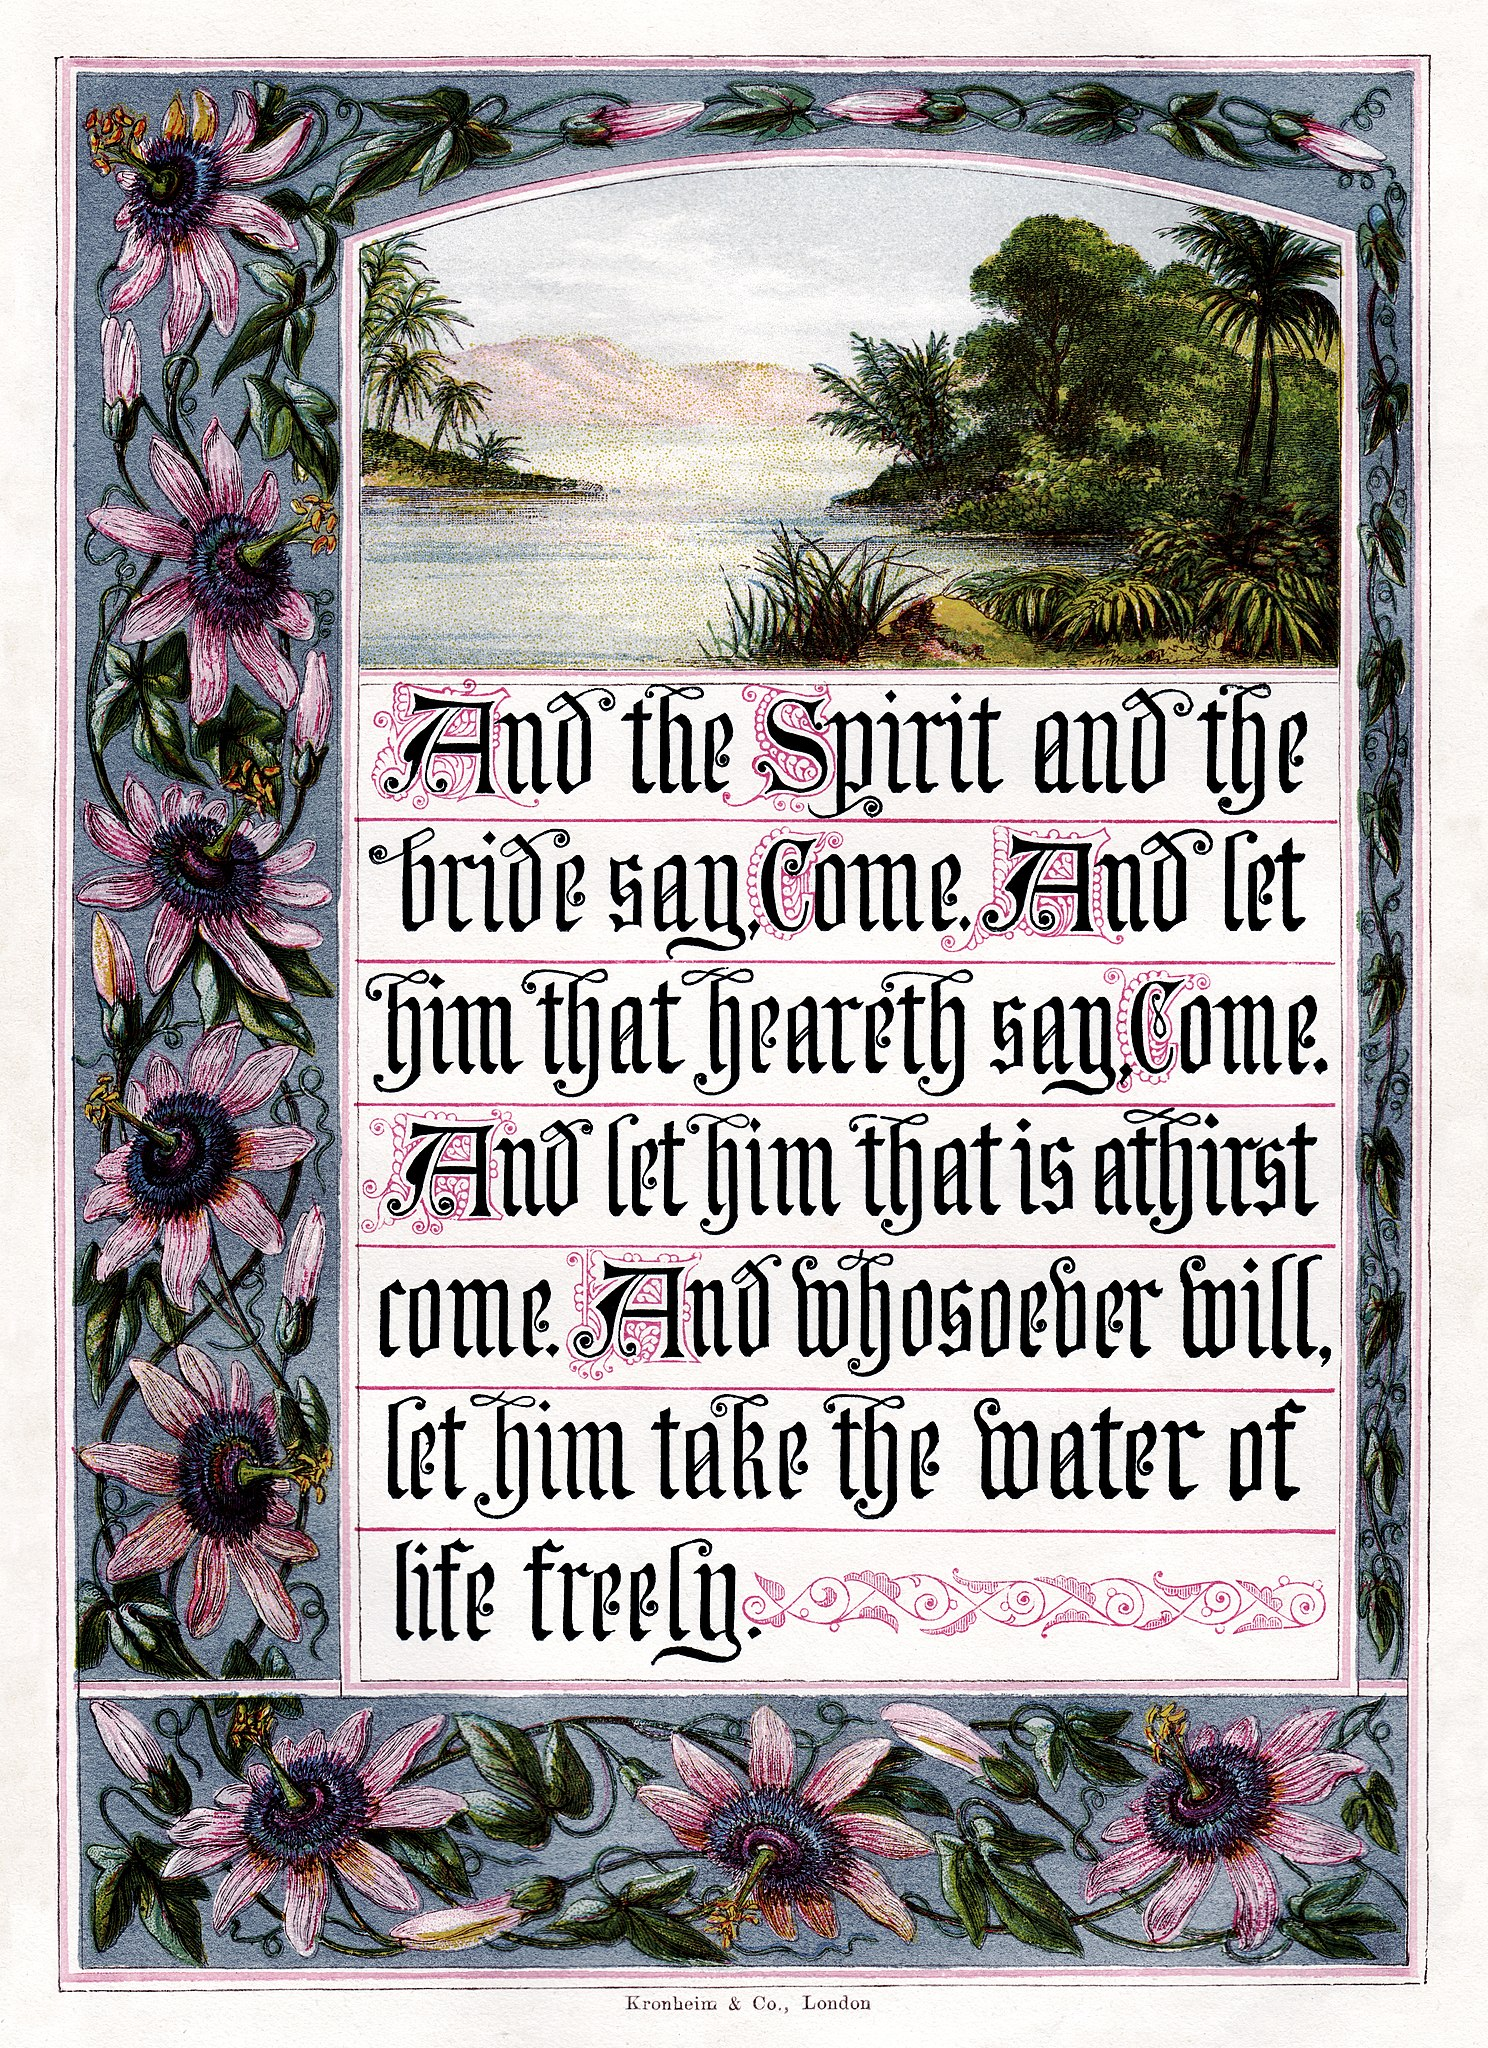
\includegraphics[width=1\textwidth]{images/illustrations/kronheimquote}
\end{center}
